\section{Ponte H}
Os motores de corrente contínua trabalham nos dois sentidos de rotação quando invertidas suas polaridades. A ponte H é um circuito que tem a função de controlar esse sentido de rotação do motor a partir da inversão de sua polaridade. O exemplo a seguir, ilustra uma ponte H composta de quatro transístores que trabalham em pares nas diagonais. Basicamente, quando se aciona uma chave tem-se 12V e a outra chave-par leva o terra (0V) para o motor. A utilização de transístores NPN e PNP é aconselhável para evitar uma perda de tensão maior entre eles, dessa forma, a carga (motor) fica sempre ligado aos coletores dos transístores.     

\begin{figure}[H]
	\centering
	\includegraphics[width=5cm]{figuras/ponteH.png}
	\caption{Representação ponte H}
	\label{ponte H}
\end{figure}

Para o projeto Green House, será necessária a confecção de uma ponte H para controle da rotação do motor. Foi realizada uma simulação no Proteus®, afim de garantir a tensão de 12V para carga, a funcionalidade do circuito e demonstrada também a entrada do controlador de operações (representado pelos 3,3V):

\begin{figure}[H]
	\centering
	\includegraphics[width=7cm]{figuras/simulacaoPonteH.png}
	\caption{Simulação da ponte H com acionamento em Q1 e Q4. Fonte: Proteus*.}
	\label{simulação ponte H}
\end{figure}

\begin{figure}[H]
	\centering
	\includegraphics[width=7cm]{figuras/simulacaoPonteH2.png}
	\caption{Simulação da ponte H com acionamento em Q2 e Q3. Fonte: Proteus*.}
	\label{simulação ponte H 2}
\end{figure}

O microcontrolador que será utilizado é uma Raspberry que trabalha com 3,3V e tem limitação na corrente de 50mA, quando utilizadas todas as suas entradas. Assim, para que essa restrição seja limitada, no nó de conexão entre o transístor e o controlador, a corrente foi limitada a 0,005mA. Para isso ocorrer, é necessário o uso de resistências de 520$\Omega$, como demonstrado a seguir:

\begin{center}
	
$\frac{V_{cc} - V_{be}}{R}$ = $l_{b}$ \\
$\frac{3,3 - 0,7}{R}$ = 0,005\\
R = 520$\Omega$\\
$I_{ce}$ = 1000 $\Omega$ * 0,005 = 5 \textit{A}

\end{center}

Onde,
\begin{itemize}

	\item Ib = corrente que aciona o transistor;
	
	\item R = resistências que serão utilizadas para controle da corrente Ib;
	
	\item $I_{ce}$ = corrente disponível à carga;
	
	\item ${V_{cc} - V_{be}}$ = diferença de tensão entre o controlador e o transístor.
	
	\item A corrente $I_{ce}$ é multiplicada por 1000 devido ao transistor TIP. Sendo ela fornecida pela fonte que será construída mais adiante.
	
\end{itemize}

Para a construção dessa ponte H, serão necessários:
\begin{itemize}

\item 2 transístores Darlington TIP 120;
\item 2 transístores Darlington TIP 125;
\item 4 resistências de 520$\Omega$;
\item 1 placa furada;
\item 3 Borne Conector 2 vias - entradas PCI

\end{itemize}

\section{Plantário}

Na hidroponia, o cultivo das hortaliças é feito em um lugar pequeno e que não gera resíduos no local (como quando utilizado areia ou terra). De acordo com Silva et al. [1], do grupo de fruticultura da Universidade Federal de Uberlândia, o pioneiro na aplicação da técnica de hidroponia foi Allen Cooper, no Glasshouse Crop Research Institute, na Inglaterra, em 1965. Cooper relatava que “a espessura do fluxo da solução nutritiva que passa através das raízes das plantas deve ser bastante pequeno (laminar), de tal maneira que as raízes não ficassem totalmente submergidas, faltando-lhes o necessário oxigênio” [1]. No Brasil, o método é amplamente difundido por meio de estruturas de PVC, que alocam as hortaliças e por onde flui água, que é oriunda de um reservatório e se destina ao mesmo reservatório após o caminho do plantio ser percorrido. A fim de ocupar o espaço disposto de forma otimizada, trabalhou-se para que o plantário tivesse a disposição semelhante com a reportada na imagem a seguir:

\begin{figure}[H]
	\centering
	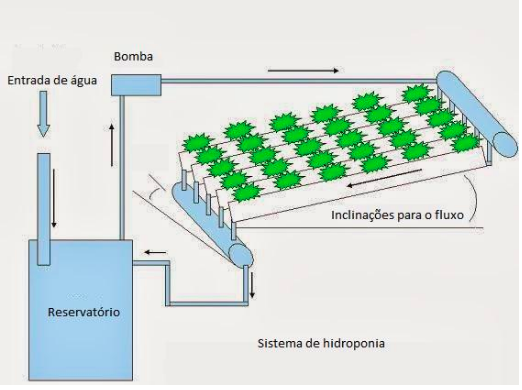
\includegraphics[width=13cm]{figuras/plantario.png}
	\caption{Plantário. Adaptado de: <http://www.ecoeficientes.com.br/o-que-e-hidroponia/hidroponia-2/}
	\label{plantario}
\end{figure}

De acordo com Silva et al. [1], a vazão ideal no para uma estrutura hidropônica está entre 1,5 litro/minuto e 2,0 litros/minuto por canaleta de cultivo.

\section{Ventilação}
Estufas são espaços fechados a fim de não sofrerem as variações de temperatura, umidade e outros fenômenos naturais. Visto que a hortaliça da Green House é definida como a alface e sua faixa de temperatura para cultivo é consideravelmente extensa (10 a 24ºC) [2], não há a necessidade de um método para aumento de temperatura e, sim, resfriamento. Com intuito de unir duas soluções, ventilação e controle de temperatura, foi definido o uso de coolers para reciclar o ar no interior da estufa, auxiliando no ajuste de umidade e na variação de temperatura. A seleção do cooler envolve apenas a variável tempo, já que o fluxo de ar a ser reciclado variará de acordo com a vazão do aparelho. A fim de poupar gastos, foram selecionados dois coolers que os integrantes já detinham para entrada de fluxo e saída de fluxo (exaustor), ambos de 12V DC. Um deles é da marca Leadership e funciona com as seguintes especificações:

\begin{itemize}
	\item Corrente: 0,12A;
	\item Dimensões: 80x80x25mm;
	\item Vazão volumétrica: 40,32 m³/h;
	\item Velocidade: 2200 RPM  
\end{itemize}

O segundo ventilador é da marca Adasa e suas condições de operação são:

\begin{itemize}
	\item Corrente: 0,08A;
	\item Dimensões: 120x120x25mm;
	\item Vazão volumétrica: 75,9 m³/h;
	\item Velocidade: 1400 RPM 
\end{itemize}

\section{Iluminação}
A iluminação artificial para plantas como alface pode parecer uma ideia infundada a primeira vista para pessoas residentes em países do sul que possuem grandes quantidades de terra disponíveis para o plantio e Iluminação abundante, porém para ambientes de temperatura muito agressiva ou Países como Japão em que a quantidade de terras disponíveis para agricultura é reduzida, ou até mesmo em espaçonaves testadas pela NASA, o uso de fontes artificiais de luz estão sendo cada vez mais desenvolvidas e aperfeiçoadas para reproduzir a luz do sol.Dessa forma vários estudos contemplam as questões nas quais são pertinentes ao projeto desenvolvido pelo grupo.

Parâmetros Utilizados no Meio

\textbf{Photosynthetic Photon Flux (PPF)}\\
É o Fluxo de Fótons mais relevantes para a fotossíntese dado em $\mu$mol $s^{-1}$, representa o número de Fótons enviados emitidos. \\
Obtida pela fórmula da energia de um fóton

\begin{flushleft}
	
	E$\lambda$=hc \\
	E= Energia 1 fóton em j \\
	Temos W= j/s
	
\end{flushleft}

Dessa forma pode ser calculado o número de prótons para uma lâmpada de 1W ao se aproximar a uma curva normal.

\begin{figure}[H]
	\centering
	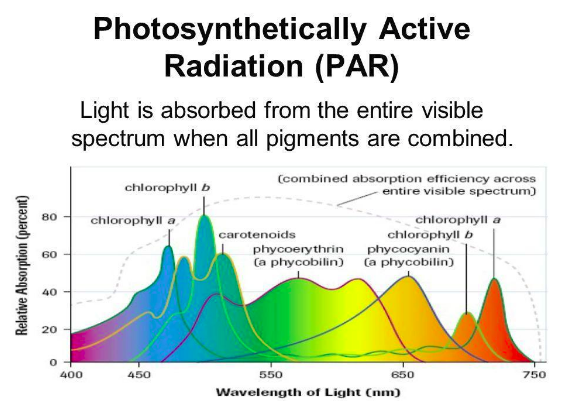
\includegraphics[width=15cm]{figuras/parGraphic.png}
	\caption{PAR(Radiação fotossinteticamente ativa)} \label{PAR}
\end{figure}

\textbf{Photosynthetic Photon Flux Density (PPFD)}\\
É o valor PPF medido por área na qual a luz projetada.Estudos acompanhados de medições por equipamentos como estes demonstram melhor qualidade em plantas que possuem PPFD  próximos a 250$\mu$mol $m^{-2}$$s^{-1}$, entretanto o valor do equipamento e elevado.

\begin{figure}[H]
	\centering
	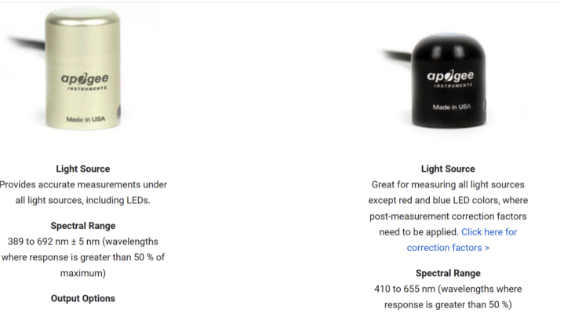
\includegraphics[width=15cm]{figuras/valor_par.png}
	\caption{Valor de U\$500 o medidor PAR/PPFD)} \label{valor_par}
\end{figure}

\begin{figure}[H]
	\centering
	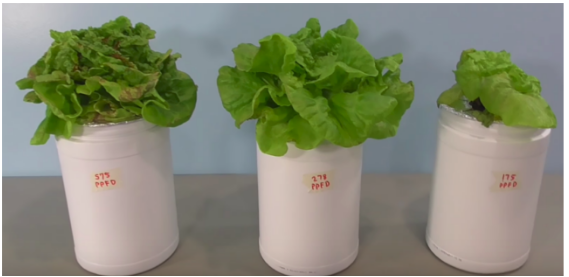
\includegraphics[width=15cm]{figuras/variacao_ppfd.png}
	\caption{Variação PPFD, qualidade de plantas com fornecimento entre 575 $\mu$mol $m^{-2}$$s^{-1}$, 278 $\mu$mol $m^{-2}$$s^{-1}$ e ,175 $\mu$mol $m^{-2}$$s^{-1}$ PPFD demonstrando ser um parâmetro quantitativo validado para ser usado.)} \label{variação_ppfd}
\end{figure}

\textbf{Lâmpadas de Vapor de sódio}

As lâmpadas de vapor de sódio de alta pressão (HPS), utilizadas para iluminação de estufas e de câmaras de crescimento de plantas dado que a sua emissão se centra em torno da região espectral de maior eficiência fotossintética, permitindo a produção de elevadas intensidades luminosas com um baixo custo energético.

\textbf{LED}

Luz Vermelha (630 -660 nm) é essencial para o crescimento das hastes, bem como a expansão das folhas. Este comprimento de onda também regula a floração, os períodos de dormência e a germinação das sementes. 

\begin{table}[H]
	\centering
	\begin{tabular}{|c|c|c|c|}
		\hline
		\multirow{2}{*}{PART NO}      & \multicolumn{2}{c|}{Chip} & \multirow{2}{*}{Lens Color} \\ \cline{2-3}
		&      Material     &     Emitted Colors	      &                   \\ \hline
		\multicolumn{1}{|l|}{LED-P1-D-Red} &   GaAllnP        &     Red      &      WATER CLEAR             \\ \hline
	\end{tabular}
	\caption{Tabela luz vermelha}
	\label{Tabela luz vermelha}
\end{table}


\begin{figure}[H]
	\centering
	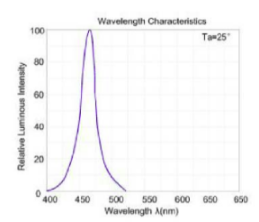
\includegraphics[width=5cm]{figuras/curva400-500.png}
	\caption{Curva característica onda} \label{curva característica 400 500}
\end{figure}

\begin{figure}[H]
	\centering
	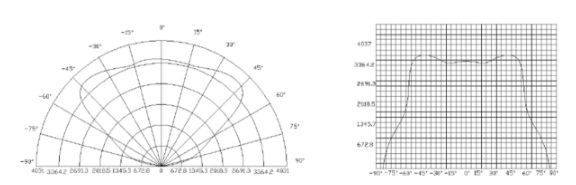
\includegraphics[width=15cm]{figuras/curva_fotometrica.png}
	\caption{curva fotométrica} \label{curva fotometrica}
\end{figure}

A Luz Azul (400 -520 nm) precisa ser cuidadosamente misturada com luz em outros espectros, pois a superexposição à luz neste comprimento de onda pode prejudicar o crescimento de certas espécies de plantas. A luz na faixa azul também afeta o conteúdo de clorofila presente na planta, bem como a espessura da folha.

\begin{figure}[H]
	\centering
	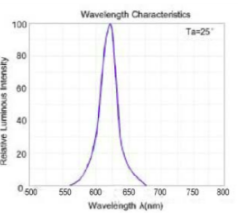
\includegraphics[width=5cm]{figuras/curva500-700.png}
	\caption{Curva característica onda} \label{curva característica 500 700}
\end{figure}

\begin{figure}[H]
	\centering
	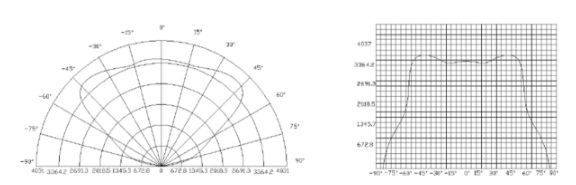
\includegraphics[width=15cm]{figuras/curva_fotometrica.png}
	\caption{curva fotométrica} \label{curva fotometrica}
\end{figure}


A luz verde (500 - 600 nm) já foi considerada não necessária para as plantas, mas estudos recentes descobriram que este comprimento de onda penetra através dos topos de folhagens  para suportar as folhas na parte inferior.


Infravermelho (720 - 740 nm) também passa por folhagens superiores densas para suportar o crescimento de folhas localizadas mais baixas nas plantas. Além disso, a exposição à luz infravermelha reduz o tempo que uma planta precisa para florescer. Outro benefício da luz vermelha distante é que as plantas expostas a este comprimento de onda tendem a produzir folhas maiores do que aquelas não expostas à luz neste espectro.


Luz Branca (400 - 650nm)

\begin{figure}[H]
	\centering
	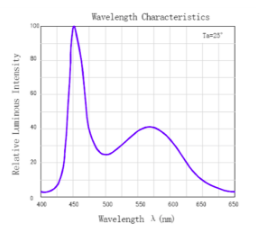
\includegraphics[width=5cm]{figuras/curva_onda.png}
	\caption{curva onda} \label{curva onda}
\end{figure}

\begin{figure}[H]
	\centering
	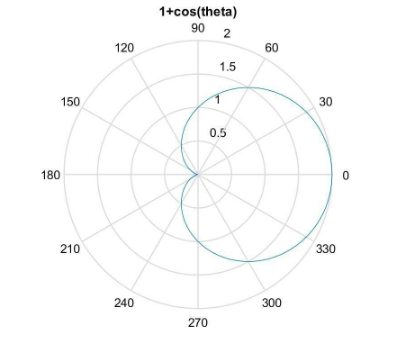
\includegraphics[width=10cm]{figuras/Cardioide.png}
	\caption{Cardioide} \label{Cardioide}
\end{figure}

UV \& IR
Presença do Infravermelho devido ao Emerson Enhancement Effect que determina que a presença de luz Infravermelha eleva a produção das clorofilas.

UV

\begin{enumerate}
	
	\item Ativa proteção natural das plantas
	\item Extremamente letal para organismos prejudiciais à planta
	
	
\end{enumerate}

\section{Fonte}
A fonte de tensão contínua é um dispositivo eletrônico que fornece um valor de tensão fixa à  carga na qual será ligada. A fonte de tensão projetada para esse projeto é constituída basicamente de quatro partes: abaixadora, retifica, filtragem e regulação de tensão.
A parte abaixadora de tensão é constituída por um transformador que tem como função diminuir o nível de tensão da rede, neste caso de 240 Vrms para  20Vp. Essa transformação  ocorre de acordo com a relação entre o número de espiras entre a parte primária e secundária do transformador. \\
O componente de retífica é a ponte retificadora na qual transforma a tensão alternada em tensão contínua, em ligação com o capacitor de desacoplamento com função de filtrar o ruído das faixas de alimentação.

\begin{figure}[H]
	\centering
	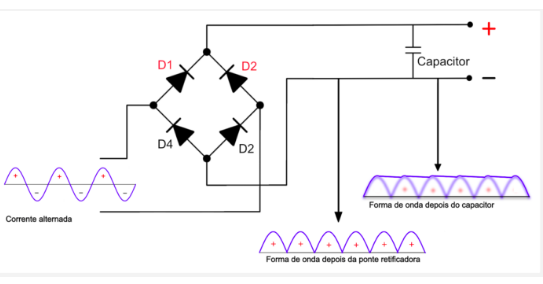
\includegraphics[width=10cm]{figuras/circuito_fonte.png}
	\caption{Circuito fonte} \label{circuito fonte}
\end{figure}

Por fim o regulador de tensão deve manter a saída constante mesmo com alterações de tensão ou corrente na saída.
